\documentclass{beamer}
\usetheme{Madrid}
\usecolortheme{default}
\usepackage[utf8]{inputenc}
\usepackage{amsmath}
\usepackage{amsfonts}
\usepackage{amssymb}
\usepackage{tikz}
\usepackage{xcolor}
\usepackage{hyperref}

\title{CRISC Exam - Hard Concepts \& Exam Traps}
\subtitle{Deep Dive Tutorial with Challenging Questions}
\author{CRISC Mastery Series}
\date{\today}

\begin{document}
	
	% ============================================================
	% TITLE SLIDE
	% ============================================================
	\begin{frame}
		\titlepage
	\end{frame}
	
	% ============================================================
	% OUTLINE
	% ============================================================
	\begin{frame}{Tutorial Outline}
		\tableofcontents
	\end{frame}
	
	% ============================================================
	% SECTION 1: RISK GOVERNANCE - BLAME CULTURE
	% ============================================================
	\section{1. Risk Governance: The Blame Culture Trap}
	
	\begin{frame}{1.1 Understanding Risk Culture}
		\begin{block}{What is Risk Culture?}
			Risk culture represents the \textbf{shared values, attitudes, and behaviors} regarding risk management within an organization.
		\end{block}
		
		\begin{alertblock}{The Critical Insight}
			Organizational behavior has a \textbf{greater impact} on risk management effectiveness than any framework, tool, or policy!
		\end{alertblock}
		
		\begin{itemize}
			\item \textbf{Healthy Risk Culture}: Open communication, learning from failures, proactive escalation
			\item \textbf{Toxic Risk Culture}: Blame, fear of reporting, hiding mistakes, finger-pointing
		\end{itemize}
	\end{frame}
	
	\begin{frame}{1.2 The Blame Culture Phenomenon}
		\begin{block}{How Blame Culture Destroys Risk Management}
			\begin{itemize}
				\item People \textbf{hide mistakes} rather than report them
				\item No one \textbf{speaks up} about emerging risks
				\item Issues escalate until they become \textbf{major incidents}
				\item \textbf{Accountability is destroyed} - no one takes ownership
				\item \textbf{Root causes} are never identified or addressed
				\item Business units \textbf{point fingers} at IT when projects fail
			\end{itemize}
		\end{block}
		
		\begin{alertblock}{The Hard Truth}
			A blame culture is the \textbf{MOST effective inhibitor} of relevant and efficient communication in any organization.
		\end{alertblock}
	\end{frame}
	
	\begin{frame}{1.3 Why Blame Culture is the Primary Concern}
		\begin{columns}
			\begin{column}{0.5\textwidth}
				\begin{block}{Consequences}
					\begin{itemize}
						\item \textbf{False sense of confidence} at top management
						\item \textbf{Perception of covering up} known risks
						\item \textbf{Misalignment} between risk appetite and policies
						\item \textbf{Inhibited communication} across all levels
						\item \textbf{Reduced risk awareness} among staff
					\end{itemize}
				\end{block}
			\end{column}
			\begin{column}{0.5\textwidth}
				\begin{exampleblock}{Key Takeaway}
					\centering
					\Large{\textbf{Address Blame Culture FIRST}}
					
					\vspace{0.3cm}
					\normalsize{Before implementing any risk management framework, tools, or policies, the organization must establish a \textbf{psychological safety} culture.}
				\end{exampleblock}
			\end{column}
		\end{columns}
	\end{frame}
	
	\begin{frame}{1.4 Overconfidence as a Culture Symptom}
		\begin{block}{The Overconfidence Trap}
			When business units believe "our teams can handle any issue that arises without additional controls," this is a \textbf{problematic risk culture} indicator.
		\end{block}
		
		\begin{itemize}
			\item Overconfidence $\rightarrow$ dismissed risk findings
			\item Dismissed findings $\rightarrow$ inadequate controls
			\item Inadequate controls $\rightarrow$ underestimated exposure
		\end{itemize}
		
		\begin{alertblock}{Exam Clue}
			Any answer showing \textbf{dismissal of risk information} or \textbf{resistance to challenge} points to a \textbf{weak risk culture}, not maturity or communication.
		\end{alertblock}
	\end{frame}
	
	% ============================================================
	% SECTION 2: 3 LINES OF DEFENSE - ROLES TRAP
	% ============================================================
	\section{2. 3 Lines of Defense: The Roles Trap}
	
	\begin{frame}{2.1 Understanding the Three Lines Model}
		\begin{block}{The Three Lines of Defense}
			\begin{tabular}{|p{2.5cm}|p{4cm}|p{4cm}|}
				\hline
				\textbf{Line} & \textbf{Who} & \textbf{Primary Responsibility} \\
				\hline
				\textbf{1st Line} & Operational Management & Own and manage risk; implement controls \\
				\hline
				\textbf{2nd Line} & Risk Oversight Functions & Monitor, challenge, and provide guidance \\
				\hline
				\textbf{3rd Line} & Internal Audit & Provide independent assurance \\
				\hline
			\end{tabular}
		\end{block}
		
		\begin{alertblock}{The Critical Insight}
			Each line has \textbf{distinct, non-overlapping responsibilities}. Confusing these roles is a \textbf{major exam trap}!
		\end{alertblock}
	\end{frame}
	
	\begin{frame}{2.2 Common Role Confusion Traps}
		\begin{block}{Trap \#1: Who Owns Risk?}
			\begin{itemize}
				\item \textbf{Common Mistake}: Thinking IT owns technology risk
				\item \textbf{Correct}: \textbf{Business management} owns all risk
				\item \textbf{Why}: Risk impacts business objectives; IT is an enabler
			\end{itemize}
		\end{block}
		
		\begin{block}{Trap \#2: Who Establishes Framework?}
			\begin{itemize}
				\item \textbf{Common Mistake}: Thinking internal audit establishes risk framework
				\item \textbf{Correct}: \textbf{Second Line} establishes and maintains framework
				\item \textbf{Why}: Framework is an oversight function, not assurance function
			\end{itemize}
		\end{block}
	\end{frame}
	
	\begin{frame}{2.3 Role Responsibilities Table}
		\begin{table}
			\centering
			\begin{tabular}{|p{2.5cm}|p{3.5cm}|p{5cm}|}
				\hline
				\textbf{Role} & \textbf{Line of Defense} & \textbf{Key Responsibilities} \\
				\hline
				Risk Owner & 1st Line & Identifies, assesses, responds to risk \\
				\hline
				Control Owner & 1st Line & Implements and maintains controls \\
				\hline
				Risk Manager & 2nd Line & Monitors risk; provides oversight \\
				\hline
				CRO & 2nd Line & Oversees risk management program \\
				\hline
				Internal Audit & 3rd Line & Provides independent assurance \\
				\hline
				Board & Governance & Sets risk appetite; provides direction \\
				\hline
			\end{tabular}
		\end{table}
		
		\begin{exampleblock}{Memory Aid}
			\textbf{First = "Do It"} | \textbf{Second = "Watch It"} | \textbf{Third = "Check It"}
		\end{exampleblock}
	\end{frame}
	
	\begin{frame}{2.4 What Happens When Lines Don't Work Together}
		\begin{block}{Symptoms of Dysfunction}
			\begin{itemize}
				\item \textbf{Each line planning independently} - Most dangerous sign
				\item Overlap in responsibilities causing confusion
				\item Gaps where no one takes ownership
				\item Duplicate work across lines
				\item Conflict between lines regarding authority
			\end{itemize}
		\end{block}
		
		\begin{alertblock}{The Critical Risk}
			When the three lines of defense don't work together effectively, the organization has \textbf{no integrated risk management} capability. Risks fall through the cracks.
		\end{alertblock}
	\end{frame}
	
	\begin{frame}{2.5 CRO Responsibility Trap}
		\begin{block}{What the CRO Actually Does}
			\begin{itemize}
				\item Manages the \textbf{risk assessment process}
				\item Ensures \textbf{corrective actions} are implemented
				\item Manages the \textbf{supporting risk management function}
				\item Provides \textbf{oversight, guidance, governance, coordination}
			\end{itemize}
		\end{block}
		
		\begin{alertblock}{The CRO Trap}
			Students select the CRO because the title contains "Risk." But the CRO \textbf{does not own business risk} and \textbf{does not accept risk} on behalf of the business.
			
			\textbf{Accountability for risk always stays with business management.}
		\end{alertblock}
	\end{frame}
	
	\begin{frame}{2.6 Data Owner vs Data Custodian}
		\begin{columns}
			\begin{column}{0.5\textwidth}
				\begin{block}{Data Owner (1st Line)}
					\begin{itemize}
						\item Classifies information
						\item Approves access and entitlements
						\item Reviews user access
						\item Determines protection requirements
						\item Provides risk perspective
					\end{itemize}
				\end{block}
			\end{column}
			\begin{column}{0.5\textwidth}
				\begin{block}{Data Custodian (Operational)}
					\begin{itemize}
						\item Implements controls
						\item Platform security
						\item Intrusion detection
						\item Antivirus controls
						\item Backups and maintenance
					\end{itemize}
				\end{block}
			\end{column}
		\end{columns}
		
		\begin{exampleblock}{Exam Rule}
			\textbf{Owner = Decides WHO gets access. Custodian = HOW systems are secured.}
		\end{exampleblock}
	\end{frame}
	
	% ============================================================
	% SECTION 3: RISK APPETITE vs TOLERANCE vs CAPACITY
	% ============================================================
	\section{3. Risk Appetite vs Tolerance vs Capacity}
	
	\begin{frame}{3.1 The Three Risk Concepts}
		\begin{block}{Concept Definitions}
			\begin{tabular}{|p{3cm}|p{8cm}|}
				\hline
				\textbf{Concept} & \textbf{Definition} \\
				\hline
				\textbf{Risk Appetite} & Amount of risk an organization is \textbf{willing to accept} in pursuit of its mission \\
				\hline
				\textbf{Risk Tolerance} & \textbf{Acceptable level of variation} from risk appetite for a specific risk \\
				\hline
				\textbf{Risk Capacity} & \textbf{Maximum risk} an organization can absorb before existence is threatened \\
				\hline
			\end{tabular}
		\end{block}
		
		\begin{alertblock}{The Critical Distinction}
			\textbf{Appetite} = \textit{Willing to take} \\
			\textbf{Tolerance} = \textit{Acceptable deviation} \\
			\textbf{Capacity} = \textit{Can survive}
		\end{alertblock}
	\end{frame}
	
	\begin{frame}{3.2 The Hierarchy Relationship}
		\begin{center}
			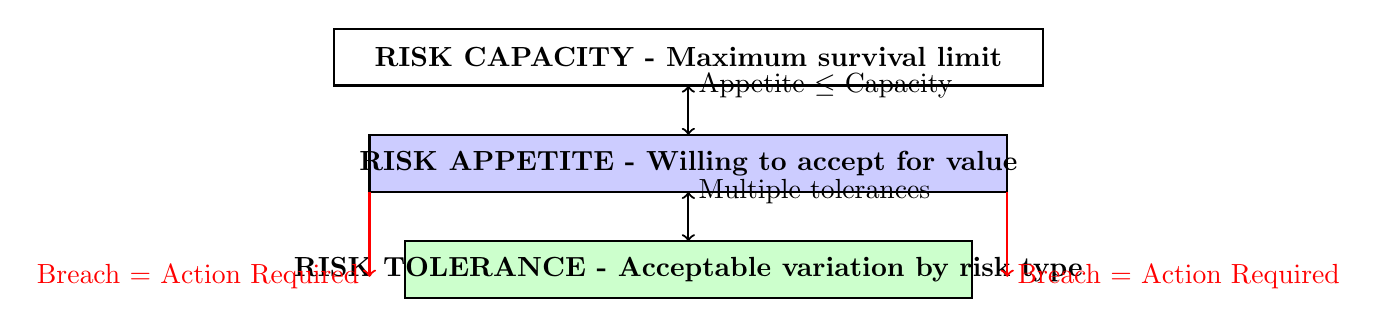
\begin{tikzpicture}[scale=0.9]
				\draw[thick] (0,0) rectangle (10,0.8) node[midway] {\textbf{RISK CAPACITY - Maximum survival limit}};
				\draw[thick, fill=blue!20] (0.5,-1.5) rectangle (9.5,-0.7) node[midway] {\textbf{RISK APPETITE - Willing to accept for value}};
				\draw[thick, fill=green!20] (1,-3) rectangle (9,-2.2) node[midway] {\textbf{RISK TOLERANCE - Acceptable variation by risk type}};
				
				\draw[<->, thick] (5,-2.2) -- (5,-1.5) node[right] {Multiple tolerances};
				\draw[<->, thick] (5,-0.7) -- (5,0) node[right] {Appetite $\le$ Capacity};
				
				\draw[->, thick, red] (0.5,-1.5) -- (0.5,-2.7) node[left] {Breach = Action Required};
				\draw[->, thick, red] (9.5,-1.5) -- (9.5,-2.7) node[right] {Breach = Action Required};
			\end{tikzpicture}
		\end{center}
	\end{frame}
	
	\begin{frame}{3.3 Common Confusion Traps}
		\begin{block}{Trap \#1: Appetite vs Tolerance}
			\begin{itemize}
				\item \textbf{Common Mistake}: Using "risk appetite" and "risk tolerance" interchangeably
				\item \textbf{Correct}: Appetite is \textbf{broad} organizational willingness; tolerance is \textbf{specific} acceptable deviation
				\item \textbf{Example}: Appetite = "We accept moderate risk for growth"; Tolerance = "15\% project cost overrun is acceptable"
			\end{itemize}
		\end{block}
		
		\begin{block}{Trap \#2: Tolerance vs Capacity}
			\begin{itemize}
				\item \textbf{Common Mistake}: Thinking tolerance breach is existential
				\item \textbf{Correct}: \textbf{Tolerance breach} requires management action; \textbf{Capacity breach} threatens existence
				\item \textbf{Example}: Projects exceed timeline by 15\% = tolerance; Bankruptcy = capacity
			\end{itemize}
		\end{block}
	\end{frame}
	
	\begin{frame}{3.4 Example Scenarios}
		\begin{block}{Scenario 1: Project Cost Overrun}
			\begin{itemize}
				\item Management advises 10\% deviation acceptable
				\item Projects currently exceeding budgets by nearly 10\%
				\item \textbf{This represents}: \textbf{Risk Tolerance} - acceptable deviation from risk appetite
			\end{itemize}
		\end{block}
		
		\begin{block}{Scenario 2: Major Financial Loss}
			\begin{itemize}
				\item Enterprise faces potential \$50M loss
				\item Enterprise can absorb up to \$100M in losses
				\item \textbf{This represents}: \textbf{Risk Capacity} - maximum before existence threatened
			\end{itemize}
		\end{block}
	\end{frame}
	
	\begin{frame}{3.5 Why Appetite Aligns with Business Objectives}
		\begin{block}{The Purpose of Alignment}
			Risk appetite aligned with business objectives allows the enterprise to \textbf{evaluate and deploy valuable resources toward objectives where risk tolerance is low}.
		\end{block}
		
		\begin{alertblock}{Common Wrong Answers}
			\begin{itemize}
				\item "Major risk is identified and eliminated" - Risk elimination is rarely cost-effective
				\item "IT and business goals are aligned" - Too narrow; appetite spans the enterprise
				\item "Risk strategy is adequately communicated" - Communication does not depend on alignment
			\end{itemize}
		\end{alertblock}
		
		\begin{exampleblock}{Exam Rule}
			Strategy Drives Appetite $\rightarrow$ Appetite Drives Investment $\rightarrow$ Investment Drives Controls.
		\end{exampleblock}
	\end{frame}
	
	% ============================================================
	% SECTION 4: CONTROL CATEGORIES
	% ============================================================
	\section{4. Control Categories: Design vs Function}
	
	\begin{frame}{4.1 Control Type Overview}
		\begin{block}{Five Control Categories}
			\begin{tabular}{|p{2.5cm}|p{4cm}|p{4.5cm}|}
				\hline
				\textbf{Type} & \textbf{Timing} & \textbf{Example} \\
				\hline
				\textbf{Preventive} & Before event & Firewall, Encryption, Training, MFA \\
				\hline
				\textbf{Detective} & During/After event & IDS, SIEM, Log monitoring, Audit trails \\
				\hline
				\textbf{Corrective} & After event & Backup restore, Incident response \\
				\hline
				\textbf{Deterrent} & Before event & Security cameras, Warning banners \\
				\hline
				\textbf{Compensating} & Ongoing & Additional oversight, Segregation \\
				\hline
			\end{tabular}
		\end{block}
		
		\begin{alertblock}{The Critical Insight}
			Control \textbf{type} describes \textbf{when} the control operates. Control \textbf{function} describes \textbf{what} the control does.
		\end{alertblock}
	\end{frame}
	
	\begin{frame}{4.2 Common Control Type Traps}
		\begin{block}{Trap \#1: Detective vs Corrective}
			\begin{itemize}
				\item \textbf{Common Mistake}: Confusing logging (detective) with restoring (corrective)
				\item \textbf{Correct}: \textbf{IDS detects} = Detective; \textbf{Backup restore} = Corrective
				\item \textbf{Why}: Timing matters - detection happens \textit{during}; correction happens \textit{after}
			\end{itemize}
		\end{block}
		
		\begin{block}{Trap \#2: Deterrent vs Preventive}
			\begin{itemize}
				\item \textbf{Common Mistake}: Thinking cameras "prevent" intrusion
				\item \textbf{Correct}: \textbf{Security cameras} = Deterrent (discourages); \textbf{Access control} = Preventive (stops)
				\item \textbf{Why}: Deterrent works through \textit{psychology}; Preventive works through \textit{mechanics}
			\end{itemize}
		\end{block}
	\end{frame}
	
	\begin{frame}{4.3 Control Example Matrix}
		\begin{table}
			\centering
			\begin{tabular}{|p{3cm}|p{4cm}|p{4cm}|}
				\hline
				\textbf{Control Example} & \textbf{Type} & \textbf{Why} \\
				\hline
				Firewall rules & Preventive & Stops unauthorized access \\
				\hline
				IDS alerts & Detective & Identifies violations \\
				\hline
				System backup & Corrective & Restores after failure \\
				\hline
				Security cameras & Deterrent & Discourages intruders \\
				\hline
				Manual approval for access & Compensating & Makes up for missing logical control \\
				\hline
				MFA & Preventive & Stops unauthorized access \\
				\hline
				SIEM log review & Detective & Identifies suspicious activity \\
			\end{tabular}
		\end{table}
	\end{frame}
	
	\begin{frame}{4.4 Post-Incident Control Categories}
		\begin{block}{Controls Used AFTER an Incident}
			\begin{itemize}
				\item \textbf{Detective} controls identify that the incident occurred
				\item \textbf{Corrective} controls fix or restore after the incident
			\end{itemize}
		\end{block}
		
		\begin{alertblock}{Exam Pattern}
			If the question says "after the incident has happened," the answer set is \textbf{Detective + Corrective} - not deterrent, not preventive, not compensating.
		\end{alertblock}
		
		\begin{exampleblock}{Compensating Control Clue}
			"Logical controls are not implemented" or "legacy system cannot support the control" $\rightarrow$ \textbf{Compensating control}.
		\end{exampleblock}
	\end{frame}
	
	\begin{frame}{4.5 Control Effectiveness vs Operation}
		\begin{block}{Two Different Questions}
			\textbf{Is the control working?} = Operational effectiveness \\
			\textbf{Is risk actually reduced?} = Control effectiveness
		\end{block}
		
		\begin{alertblock}{CRISC Exam Distinction}
			Control monitoring exists to verify whether the control is \textbf{effectively addressing the risk} - not merely whether the control itself is running.
		\end{alertblock}
		
		\begin{exampleblock}{Key Evidence}
			\textbf{Testing that demonstrates achievement of control objectives} is the BEST evidence of control effectiveness. \\
			Reliability, automated failure notification, and design documentation are secondary.
		\end{exampleblock}
	\end{frame}
	
	% ============================================================
	% SECTION 5: RISK RESPONSE STRATEGIES
	% ============================================================
	\section{5. Risk Response Strategies}
	
	\begin{frame}{5.1 The Four Response Strategies}
		\begin{block}{Negative Risk Responses}
			\begin{tabular}{|p{2.5cm}|p{4cm}|p{5cm}|}
				\hline
				\textbf{Strategy} & \textbf{Action} & \textbf{Example} \\
				\hline
				\textbf{Avoid} & Eliminate risk & Terminate project; don't engage \\
				\hline
				\textbf{Mitigate} & Reduce probability/impact & Implement controls; add safeguards \\
				\hline
				\textbf{Transfer} & Shift risk to third party & Insurance; outsourcing \\
				\hline
				\textbf{Accept} & Take no action & Acknowledge and monitor \\
				\hline
			\end{tabular}
		\end{block}
		
		\begin{alertblock}{The Critical Insight}
			\textbf{Avoid} is the \textbf{only strategy} that eliminates risk entirely. All other strategies leave some residual risk.
		\end{alertblock}
	\end{frame}
	
	\begin{frame}{5.2 Positive Risk Responses}
		\begin{block}{Opportunity Responses}
			\begin{tabular}{|p{2.5cm}|p{4cm}|p{5cm}|}
				\hline
				\textbf{Strategy} & \textbf{Action} & \textbf{Example} \\
				\hline
				\textbf{Exploit} & Seize the opportunity & Pursue the beneficial outcome \\
				\hline
				\textbf{Enhance} & Increase probability/impact & Invest more to gain more \\
				\hline
				\textbf{Share} & Partner with others & Joint venture; partnership \\
				\hline
				\textbf{Accept} & Take no action & Monitor passively \\
				\hline
			\end{tabular}
		\end{block}
		
		\begin{exampleblock}{Key Distinction}
			\textbf{Exploit} = "Make it happen" | \textbf{Enhance} = "Make it more likely"
		\end{exampleblock}
	\end{frame}
	
	\begin{frame}{5.3 Response Strategy Traps}
		\begin{block}{Trap \#1: Mitigate vs Transfer}
			\begin{itemize}
				\item \textbf{Common Mistake}: Thinking outsourcing is always transfer
				\item \textbf{Correct}: \textbf{Outsourcing} is \textbf{mitigation} if risk remains; \textbf{Transfer} if contract shifts liability
				\item \textbf{Example}: Hiring IT support = mitigation; Buying insurance = transfer
			\end{itemize}
		\end{block}
		
		\begin{block}{Trap \#2: Accept vs Avoid}
			\begin{itemize}
				\item \textbf{Common Mistake}: Confusing "doing nothing" with "eliminating"
				\item \textbf{Correct}: \textbf{Avoidance} is active elimination; \textbf{Acceptance} is passive retention
				\item \textbf{Example}: Not doing e-commerce = avoid; Not fixing known vulnerability = accept
			\end{itemize}
		\end{block}
	\end{frame}
	
	\begin{frame}{5.4 Cost-Benefit Decision Framework}
		\begin{block}{Decision Logic}
			\begin{itemize}
				\item \textbf{If Cost of Control < Expected Loss}: Implement control (Mitigate)
				\item \textbf{If Cost of Control > Expected Loss}: Accept risk or Transfer
				\item \textbf{If Risk Exceeds Risk Appetite}: Must Mitigate or Transfer
				\item \textbf{If Risk Exceeds Risk Capacity}: Must Avoid
			\end{itemize}
		\end{block}
		
		\begin{exampleblock}{Classic Exam Scenario}
			Anti-malware cost exceeds loss expectancy of malware threats.
			
			\textbf{Most viable response}: Risk Acceptance
			
			\textbf{Why?} When cost of mitigation exceeds expected loss, the business case doesn't justify spending.
		\end{exampleblock}
	\end{frame}
	
	\begin{frame}{5.5 Response Recognition Pattern}
		\begin{block}{Read the Verb, Find the Response}
			\begin{tabular}{|p{4.5cm}|p{4cm}|}
				\hline
				\textbf{Question Language} & \textbf{Response} \\
				\hline
				"Purchases insurance" & Transfer / Share \\
				\hline
				"Implements MFA / cross-training" & Mitigate \\
				\hline
				"Decides not to proceed / cancel" & Avoid \\
				\hline
				"Knowingly retains residual risk" & Accept \\
				\hline
				"Profitable byproduct is realized" & Exploit \\
				\hline
				"Partners with another party" & Share (opportunity) \\
				\hline
			\end{tabular}
		\end{block}
		
		\begin{alertblock}{Trap}
			"Treat" is sometimes used loosely but is \textbf{not a formal CRISC response strategy}. The four formal strategies are Accept, Mitigate, Transfer, Avoid.
		\end{alertblock}
	\end{frame}
	
	\begin{frame}{5.6 When to Accept Risk}
		\begin{block}{Acceptance Criteria}
			Risk should be accepted when it \textbf{falls within organizational risk appetite and tolerance}.
		\end{block}
		
		\begin{itemize}
			\item \textbf{Incorrect}: "When it exceeds risk capacity" - must avoid or treat
			\item \textbf{Incorrect}: "When controls are available" - consider mitigation
			\item \textbf{Incorrect}: "When cost of controls is low" - low cost may justify mitigation
		\end{itemize}
		
		\begin{alertblock}{Risk Avoidance Defined}
			Avoidance means \textbf{exiting the activities or conditions that give rise to risk}. It is the choice that remains when no other response is adequate.
		\end{alertblock}
	\end{frame}
	
	\begin{frame}{5.7 Insurance and Trigger Recognition}
		\begin{block}{Transfer Through Insurance}
			Insurance is the classic \textbf{risk transfer} / risk sharing response. The organization still experiences the event, but the financial burden is shared with the insurer.
		\end{block}
		
		\begin{block}{Risk Trigger}
			A \textbf{trigger} is a warning sign that a risk event is about to occur (e.g., "vendor calls to say delivery won't arrive on time").
		\end{block}
		
		\begin{exampleblock}{Decision Tree Tool}
			To \textbf{choose among multiple response alternatives}, use \textbf{decision tree analysis} (probability, impact, expected outcome).
		\end{exampleblock}
	\end{frame}
	
	% ============================================================
	% SECTION 6: QUALITATIVE vs QUANTITATIVE ANALYSIS
	% ============================================================
	\section{6. Qualitative vs Quantitative Analysis}
	
	\begin{frame}{6.1 Analysis Methods Comparison}
		\begin{block}{Qualitative Risk Analysis}
			\begin{itemize}
				\item \textbf{Approach}: Subjective, judgment-based
				\item \textbf{Scale}: High/Medium/Low or 1-5 ratings
				\item \textbf{Cost}: Less expensive, faster
				\item \textbf{Output}: Risk ranking, priority list
				\item \textbf{Best For}: Initial screening, where data is scarce
			\end{itemize}
		\end{block}
		
		\begin{block}{Quantitative Risk Analysis}
			\begin{itemize}
				\item \textbf{Approach}: Statistical, data-driven
				\item \textbf{Scale}: Monetary values, percentages
				\item \textbf{Cost}: More expensive, complex
				\item \textbf{Output}: ALE, ROI, probability distributions
				\item \textbf{Best For}: High-stakes decisions, where data exists
			\end{itemize}
		\end{block}
	\end{frame}
	
	\begin{frame}{6.2 Key Formulas}
		\begin{block}{Quantitative Risk Formulas}
			\begin{itemize}
				\item \textbf{SLE} = AV × EF
				\begin{itemize}
					\item SLE = Single Loss Expectancy
					\item AV = Asset Value
					\item EF = Exposure Factor (\% loss from single event)
				\end{itemize}
				\item \textbf{ALE} = SLE × ARO
				\begin{itemize}
					\item ALE = Annualized Loss Expectancy
					\item ARO = Annualized Rate of Occurrence
				\end{itemize}
				\item \textbf{Residual Risk} = Inherent Risk × Control Risk
			\end{itemize}
		\end{block}
		
		\begin{alertblock}{Memory Aid}
			\textbf{SLE × ARO = ALE}
		\end{alertblock}
	\end{frame}
	
	\begin{frame}{6.3 Qualitative vs Quantitative Trap}
		\begin{block}{Trap: Which Method to Use?}
			\begin{itemize}
				\item \textbf{Common Mistake}: Using quantitative when data is unreliable
				\item \textbf{Correct}: Use \textbf{qualitative} when data is scarce; \textbf{quantitative} when data is available
				\item \textbf{Example}: New technology risk = qualitative; Established system loss history = quantitative
			\end{itemize}
		\end{block}
		
		\begin{block}{The Cost Trap}
			\begin{itemize}
				\item \textbf{Quantitative} is generally \textbf{more expensive} than qualitative
				\item \textbf{Common Mistake}: Thinking quantitative is always better
				\item \textbf{Correct}: Choose based on \textbf{business need}, not sophistication
				\item \textbf{Example}: ROI of controls = quantitative; Risk ranking = qualitative
			\end{itemize}
		\end{block}
	\end{frame}
	
	\begin{frame}{6.4 Statistical Analysis and Exposure Factor}
		\begin{block}{Quantitative Analysis Requires}
			\begin{itemize}
				\item Reliable loss estimates and threat frequency data
				\item Historical incident metrics and asset valuations
				\item Statistical methods to derive likelihood and impact
			\end{itemize}
		\end{block}
		
		\begin{alertblock}{Exposure Factor Boundary}
			If an asset is \textbf{completely lost}, $EF = 1.0$ (100\%). EF ranges from 0 to 1 and is never infinite.
		\end{alertblock}
		
		\begin{exampleblock}{SLE Example}
			Server worth \$100,000 completely destroyed by fire: $SLE = \$100{,}000 \times 1.0 = \$100{,}000$.
		\end{exampleblock}
	\end{frame}
	
	\begin{frame}{6.5 Analysis Techniques Roundup}
		\begin{block}{Which Technique Answers Which Question?}
			\begin{tabular}{|p{4.5cm}|p{5cm}|}
				\hline
				\textbf{Question} & \textbf{Technique} \\
				\hline
				"How did this failure happen?" (top-down) & Fault Tree Analysis \\
				\hline
				"What could happen next?" (forward) & Event Tree Analysis \\
				\hline
				"Aggregate variation across inputs" & Monte Carlo Simulation \\
				\hline
				"Visualize causes, controls, consequences" & Bow Tie Analysis \\
				\hline
				"Get anonymous expert consensus" & Delphi Technique \\
				\hline
				"Quantify risk in financial terms" & FAIR \\
				\hline
				"Asset-centric self-directed assessment" & OCTAVE \\
				\hline
			\end{tabular}
		\end{block}
	\end{frame}
	
	\begin{frame}{6.6 OCTAVE Deep Dive}
		\begin{block}{OCTAVE Essentials}
			OCTAVE = Operationally Critical Threat, Asset, and Vulnerability Evaluation
		\end{block}
		
		\begin{itemize}
			\item \textbf{Focus}: Critical assets and the risks to those assets
			\item \textbf{Phase 1}: Build \textbf{asset-based threat profiles} (organizational evaluation)
			\item \textbf{Phase 2}: Identify infrastructure vulnerabilities
			\item \textbf{Phase 3}: Develop security strategy
		\end{itemize}
		
		\begin{alertblock}{Trap}
			OCTAVE is \textbf{asset-centric and business-context-driven} - NOT primarily about technical vulnerability scanning, financial quantification, or compliance.
		\end{alertblock}
	\end{frame}
	
	\begin{frame}{6.7 Delphi, Fault Tree, and Monte Carlo}
		\begin{block}{Delphi Technique}
			Leverages \textbf{expert opinion} through \textbf{two or more rounds of anonymous questionnaires}. After each round, a facilitator summarizes results.
		\end{block}
		
		\begin{block}{Fault Tree Analysis (FTA)}
			\textbf{Top-down} analysis starting with an undesirable event and working backward to identify combinations of failures and root causes.
		\end{block}
		
		\begin{block}{Monte Carlo Analysis}
			Establishes the \textbf{aggregate variation} in a system resulting from variations in multiple inputs, each with a defined distribution.
		\end{block}
	\end{frame}
	
	\begin{frame}{6.8 Risk Identification Tools Traps}
		\begin{block}{Tool vs Phase}
			\begin{tabular}{|p{4cm}|p{4.5cm}|p{3cm}|}
				\hline
				\textbf{Tool} & \textbf{Purpose} & \textbf{Phase} \\
				\hline
				Process flowchart & Map process steps, find failure points & Identification \\
				\hline
				Ishikawa (fishbone) & Root cause analysis & Identification \\
				\hline
				Influence diagram & Show relationships/dependencies & Identification \\
				\hline
				Decision tree & Evaluate alternatives, EMV & Quantitative Analysis \\
				\hline
			\end{tabular}
		\end{block}
		
		\begin{alertblock}{Key Trap}
			\textbf{Decision tree diagrams are NOT risk identification tools} - they are used in quantitative risk analysis.
		\end{alertblock}
	\end{frame}
	
	% ============================================================
	% SECTION 7: KRI vs KPI vs KCI
	% ============================================================
	\section{7. KRI vs KPI vs KCI}
	
	\begin{frame}{7.1 Understanding the Metrics}
		\begin{block}{Three Key Metrics}
			\begin{tabular}{|p{2.5cm}|p{4cm}|p{4.5cm}|}
				\hline
				\textbf{Metric} & \textbf{Purpose} & \textbf{Example} \\
				\hline
				\textbf{KRI} & Predict future risk & \% of open critical vulnerabilities \\
				\hline
				\textbf{KPI} & Measure performance & System uptime \% \\
				\hline
				\textbf{KCI} & Measure control effectiveness & \% of access reviews completed \\
				\hline
			\end{tabular}
		\end{block}
		
		\begin{alertblock}{The Critical Insight}
			\textbf{KRIs = Early Warning Signals} - They look \textbf{forward} at emerging risk \\
			\textbf{KPIs = Performance Indicators} - They look \textbf{backward} at what happened \\
			\textbf{KCIs = Control Effectiveness} - They measure if controls are \textbf{working}
		\end{alertblock}
	\end{frame}
	
	\begin{frame}{7.2 KRI Maintenance Reason}
		\begin{block}{The Most Important Reason to Maintain KRIs}
			\begin{itemize}
				\item \textbf{Answer}: Threats and vulnerabilities change over time
				\item \textbf{Why?} Risk environment is dynamic; KRIs must evolve
				\item \textbf{Why Not?}
				\begin{itemize}
					\item Avoid risk = Risk response strategy, not maintenance
					\item Fine-tuning = Secondary concern
					\item Timeliness = Business requirement
				\end{itemize}
			\end{itemize}
		\end{block}
		
		\begin{exampleblock}{Key Understanding}
			As threats change, the indicators that predict risk \textbf{must also change}. A KRI that worked last year may be irrelevant today.
		\end{exampleblock}
	\end{frame}
	
	\begin{frame}{7.3 Common Metric Confusion}
		\begin{block}{Trap: KRI vs KPI}
			\begin{itemize}
				\item \textbf{Common Mistake}: Thinking KRIs and KPIs are the same
				\item \textbf{Correct}: \textbf{KRIs predict risk}; \textbf{KPIs measure performance}
				\item \textbf{Example}: 
				\begin{itemize}
					\item KRI: "Number of open critical vulnerabilities" = \textit{risk indicator}
					\item KPI: "Average time to patch" = \textit{performance indicator}
				\end{itemize}
			\end{itemize}
		\end{block}
		
		\begin{block}{Trap: KCI vs KRI}
			\begin{itemize}
				\item \textbf{Common Mistake}: Using KCIs as risk indicators
				\item \textbf{Correct}: \textbf{KCIs measure control operation}; \textbf{KRIs measure risk level}
				\item \textbf{Example}:
				\begin{itemize}
					\item KCI: "Firewall rules reviewed monthly" = \textit{control effectiveness}
					\item KRI: "Percentage of risky firewall rule changes" = \textit{risk indicator}
				\end{itemize}
			\end{itemize}
		\end{block}
	\end{frame}
	
	\begin{frame}{7.4 KRI Optimization: Sensitivity Trap}
		\begin{block}{Too Many False Positives?}
			If a KRI generates excessive alerts that rarely identify real risk, adjust the \textbf{sensitivity thresholds}.
		\end{block}
		
		\begin{alertblock}{Adjustment Map}
			\begin{itemize}
				\item Too many alerts $\rightarrow$ Reduce sensitivity
				\item Missed risk events $\rightarrow$ Increase sensitivity
				\item Late alerts $\rightarrow$ Improve timeliness
				\item Poor data quality $\rightarrow$ Improve reliability
			\end{itemize}
		\end{alertblock}
	\end{frame}
	
	\begin{frame}{7.5 KPI + KRI Together}
		\begin{block}{Why Monitor Both?}
			KPIs measure whether objectives are being achieved; KRIs provide insight into \textbf{increasing risk exposure}. Together they show both performance and emerging threats.
		\end{block}
		
		\begin{alertblock}{Classic Scenario}
			Dashboard showing incident response time (KPI), patch compliance (KPI/KCI), privileged-access violations (KRI), and phishing events (KRI).
		\end{alertblock}
		
		\begin{exampleblock}{Best Indicator of Detection/Response Effectiveness}
			\textbf{Average detection and response time} - not training completion, raw incident counts, or audit findings.
		\end{exampleblock}
	\end{frame}
	
	% ============================================================
	% SECTION 8: RESIDUAL vs INHERENT vs CURRENT RISK
	% ============================================================
	\section{8. Residual vs Inherent vs Current Risk}
	
	\begin{frame}{8.1 Understanding the Risk Types}
		\begin{block}{Three Risk States}
			\begin{tabular}{|p{2.5cm}|p{4cm}|p{4.5cm}|}
				\hline
				\textbf{Risk Type} & \textbf{Definition} & \textbf{When Measured} \\
				\hline
				\textbf{Inherent Risk} & Risk without controls & Before any controls \\
				\hline
				\textbf{Residual Risk} & Risk after controls & After controls implemented \\
				\hline
				\textbf{Current Risk} & Risk in real-time & At specific point in time \\
				\hline
			\end{tabular}
		\end{block}
		
		\begin{alertblock}{The Critical Insight}
			\textbf{Residual Risk} = Inherent Risk - Controls \\
			\textbf{Current Risk} = Residual Risk in a \textit{real-time threat scenario}
		\end{alertblock}
	\end{frame}
	
	\begin{frame}{8.2 The Risk Reduction Equation}
		\begin{center}
			\Large{\textbf{Inherent Risk × Control Risk = Residual Risk}}
		\end{center}
		
		\begin{block}{Understanding the Formula}
			\begin{itemize}
				\item \textbf{Inherent Risk}: Risk level before any controls
				\item \textbf{Control Risk}: Risk that controls \textit{fail} to mitigate
				\item \textbf{Residual Risk}: Risk that remains after controls
			\end{itemize}
		\end{block}
		
		\begin{exampleblock}{Key Concept}
			The \textbf{purpose} of risk mitigation is to reduce \textbf{residual risk} to acceptable levels.
			
			You cannot reduce \textbf{inherent risk} - you can only reduce the \textbf{impact} of controls failure.
		\end{exampleblock}
	\end{frame}
	
	\begin{frame}{8.3 Common Risk Type Traps}
		\begin{block}{Trap: Inherent vs Residual}
			\begin{itemize}
				\item \textbf{Common Mistake}: Thinking controls eliminate all risk
				\item \textbf{Correct}: Controls reduce risk but \textbf{never eliminate} it entirely
				\item \textbf{Why?} Residual risk always remains after controls
			\end{itemize}
		\end{block}
		
		\begin{block}{Trap: Current vs Residual}
			\begin{itemize}
				\item \textbf{Common Mistake}: Using residual and current interchangeably
				\item \textbf{Correct}: \textbf{Residual} is theoretical risk after controls; \textbf{Current} is real-time risk in actual environment
				\item \textbf{Example}: 
				\begin{itemize}
					\item Residual = Risk after firewall is deployed
					\item Current = Risk \textit{right now} with current threat intelligence
				\end{itemize}
			\end{itemize}
		\end{block}
	\end{frame}
	
	\begin{frame}{8.4 Top Risk Register Facts}
		\begin{block}{Value of the Risk Register}
			A risk register's greatest value is that it \textbf{drives the risk response plan} - not merely capturing inventory, reporting, or categorizing risks.
		\end{block}
		
		\begin{alertblock}{Risk Register Contents}
			Risk descriptions, likelihood, impact, ownership, treatment strategies, residual risk, ratings, and monitoring status.
		\end{alertblock}
		
		\begin{exampleblock}{No Register = No Prioritization = No Risk Response}
		\end{exampleblock}
	\end{frame}
	
	% ============================================================
	% SECTION 9: RPO vs RTO vs MTD
	% ============================================================
	\section{9. RPO vs RTO vs MTD}
	
	\begin{frame}{9.1 Recovery Objectives}
		\begin{block}{Three Recovery Metrics}
			\begin{tabular}{|p{2.5cm}|p{4cm}|p{4.5cm}|}
				\hline
				\textbf{Metric} & \textbf{Definition} & \textbf{Direction} \\
				\hline
				\textbf{RPO} & Maximum acceptable data loss & Backward-looking \\
				\hline
				\textbf{RTO} & Maximum acceptable downtime & Forward-looking \\
				\hline
				\textbf{MTD} & Maximum tolerated outage & Total threshold \\
				\hline
			\end{tabular}
		\end{block}
		
		\begin{alertblock}{The Critical Insight}
			\textbf{RPO} = "How much data can we lose?" \\
			\textbf{RTO} = "How long can we be down?" \\
			\textbf{MTD} = "How long before we die?"
		\end{alertblock}
	\end{frame}
	
	\begin{frame}{9.2 Understanding RPO Direction}
		\begin{block}{RPO is Backward-Looking}
			\begin{itemize}
				\item \textbf{RPO} measures \textbf{acceptable data loss} going backward in time
				\item \textbf{Example}: RPO = 4 hours means "We can accept losing 4 hours of data"
				\item \textbf{Why?} Data lost during the last 4 hours is acceptable
			\end{itemize}
		\end{block}
		
		\begin{block}{RTO is Forward-Looking}
			\begin{itemize}
				\item \textbf{RTO} measures \textbf{acceptable downtime} going forward from disruption
				\item \textbf{Example}: RTO = 2 hours means "We must be up within 2 hours"
				\item \textbf{Why?} Downtime beyond 2 hours is unacceptable
			\end{itemize}
		\end{block}
	\end{frame}
	
	\begin{frame}{9.3 Relationship Between Metrics}
		\begin{center}
			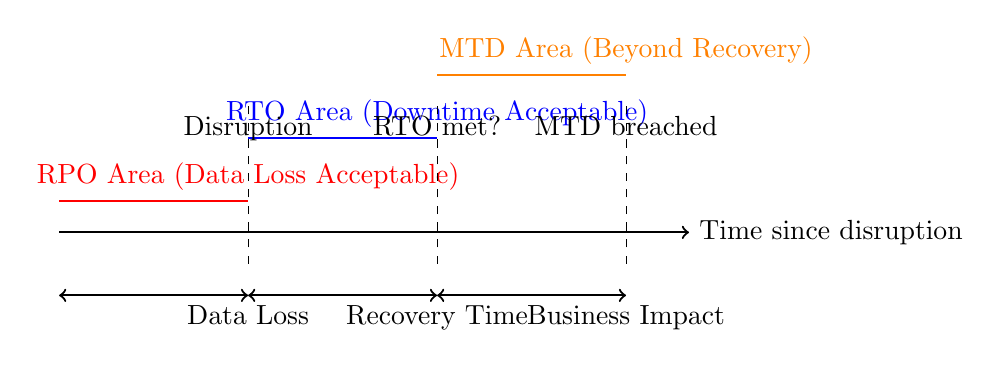
\begin{tikzpicture}[scale=0.8]
				\draw[->, thick] (0,0) -- (10,0) node[right] {Time since disruption};
				
				\draw[thick, red] (0,0.5) -- (3,0.5) node[above] {RPO Area (Data Loss Acceptable)};
				\draw[thick, blue] (3,1.5) -- (6,1.5) node[above] {RTO Area (Downtime Acceptable)};
				\draw[thick, orange] (6,2.5) -- (9,2.5) node[above] {MTD Area (Beyond Recovery)};
				
				\draw[dashed] (3,-0.5) -- (3,2) node[below] {Disruption};
				\draw[dashed] (6,-0.5) -- (6,2) node[below] {RTO met?};
				\draw[dashed] (9,-0.5) -- (9,2) node[below] {MTD breached};
				
				\draw[<->, thick] (0,-1) -- (3,-1) node[below] {Data Loss};
				\draw[<->, thick] (3,-1) -- (6,-1) node[below] {Recovery Time};
				\draw[<->, thick] (6,-1) -- (9,-1) node[below] {Business Impact};
			\end{tikzpicture}
		\end{center}
		
		\begin{exampleblock}{Key Relationship}
			RTO must be \textbf{less than} MTD. \\
			If RTO $\ge$ MTD, the business cannot recover before failure.
		\end{exampleblock}
	\end{frame}
	
	\begin{frame}{9.4 BIA vs Risk Assessment}
		\begin{block}{How They Differ}
			\begin{itemize}
				\item \textbf{BIA}: Determines business impact of disruptions and establishes recovery objectives (RTO, RPO, MTD). Asks "What happens if a process fails?"
				\item \textbf{Risk Assessment}: Evaluates threats, vulnerabilities, likelihood, and impact to determine risk levels. Asks "What causes the failure?"
			\end{itemize}
		\end{block}
		
		\begin{alertblock}{Memory Aid}
			\textbf{BIA $\rightarrow$ BCP}. BIA outputs RTO, RPO, MTD. The BCP is built using BIA results. BC/DR tests validate the completed plan.
		\end{alertblock}
	\end{frame}
	
	\begin{frame}{9.5 RTO/MTD Worked Example}
		\begin{block}{Scenario}
			Application must be recovered within 4 hours; business tolerates no more than 6 hours of total disruption.
		\end{block}
		
		\begin{itemize}
			\item \textbf{RTO = 4 hours} (recovery target)
			\item \textbf{MTD = 6 hours} (business survival limit)
			\item Rule: RTO $\le$ MTD
		\end{itemize}
		
		\begin{alertblock}{BIA Question Trap}
			If the question asks for RTO/RPO/MTD, answer \textbf{Business Impact Analysis}. Risk assessment identifies threats; BIA sets recovery targets.
		\end{alertblock}
	\end{frame}
	
	% ============================================================
	% SECTION 10: DATA OWNER vs CUSTODIAN vs USER
	% ============================================================
	\section{10. Data Owner vs Custodian vs User}
	
	\begin{frame}{10.1 Data Roles Explained}
		\begin{block}{Three Key Data Roles}
			\begin{tabular}{|p{2.5cm}|p{4cm}|p{4.5cm}|}
				\hline
				\textbf{Role} & \textbf{Responsibility} & \textbf{Example Tasks} \\
				\hline
				\textbf{Data Owner} & Classifies data; approves access & Determines sensitivity; grants permissions \\
				\hline
				\textbf{Data Custodian} & Implements controls; maintains data & Backup; encryption; security patching \\
				\hline
				\textbf{Data User} & Access data for business need & Read/update data within authorization \\
				\hline
			\end{tabular}
		\end{block}
		
		\begin{alertblock}{The Critical Insight}
			\textbf{Owner} = \textit{Decides what happens to data} \\
			\textbf{Custodian} = \textit{Protects and maintains data} \\
			\textbf{User} = \textit{Uses data for business purposes}
		\end{alertblock}
	\end{frame}
	
	\begin{frame}{10.2 Common Data Role Traps}
		\begin{block}{Trap: Data Classification}
			\begin{itemize}
				\item \textbf{Common Mistake}: Thinking the IT department classifies data
				\item \textbf{Correct}: \textbf{Data Owner} classifies data based on business criticality
				\item \textbf{Why?} IT doesn't know the business value of the data
			\end{itemize}
		\end{block}
		
		\begin{block}{Trap: Access Approval}
			\begin{itemize}
				\item \textbf{Common Mistake}: Thinking the system administrator approves access
				\item \textbf{Correct}: \textbf{Data Owner} approves access; \textbf{Custodian} implements it
				\item \textbf{Why?} Owner knows who needs access; Custodian implements technically
			\end{itemize}
		\end{block}
		
		\begin{block}{Trap: User Entitlement Changes}
			\begin{itemize}
				\item \textbf{Common Mistake}: Thinking IT decides user entitlement changes
				\item \textbf{Correct}: \textbf{Data Owner} is responsible for assigning user entitlement changes
				\item \textbf{Why?} IT implements; Owner decides
			\end{itemize}
		\end{block}
	\end{frame}
	
	\begin{frame}{10.3 Data Labeling and Classification}
		\begin{block}{Why Classification Matters}
			Data labeling supports the \textbf{entire information lifecycle}:
			\begin{itemize}
				\item Retention and archival decisions
				\item Disposal and secure destruction
				\item DLP enforcement
				\item Legal holds and access control decisions
			\end{itemize}
		\end{block}
		
		\begin{exampleblock}{Classification Example}
			Healthcare records + driver's licenses contain both PHI and PII $\rightarrow$ classify as \textbf{Sensitive}.
		\end{exampleblock}
	\end{frame}
	
	\begin{frame}{10.4 Data Security vs Data Privacy}
		\begin{block}{Key Distinction}
			\begin{itemize}
				\item \textbf{Security} = Protect the data (encryption, firewalls, access control)
				\item \textbf{Privacy} = Use the data properly (consent, lawful basis, minimization)
			\end{itemize}
		\end{block}
		
		\begin{alertblock}{The Classic Scenario}
			A bank encrypts records, restricts access, and monitors access attempts - but collects \textbf{more personal information than necessary}.
			
			\textbf{Conclusion}: Strong security does \textbf{not} guarantee privacy.
		\end{alertblock}
		
		\begin{exampleblock}{Memory Aid}
			You can have security without privacy. You \textbf{cannot} have privacy without security.
		\end{exampleblock}
	\end{frame}
	
	\begin{frame}{10.5 Privacy Compliance: Consent First}
		\begin{block}{When Using Personal Data for Marketing}
			Obtaining \textbf{appropriate customer consent} is the most important action to reduce privacy compliance risk.
		\end{block}
		
		\begin{itemize}
			\item Encryption $\rightarrow$ security, not lawful basis
			\item Firewalls $\rightarrow$ security, not lawful basis
			\item Training $\rightarrow$ supports awareness, not consent
		\end{itemize}
		
		\begin{alertblock}{Regulation Map}
			HIPAA = US health information \quad GDPR = EU residents \\
			CCPA = California residents \quad SOX = US public company financials
		\end{alertblock}
	\end{frame}
	
	% ============================================================
	% SECTION 11: CIA TRIAD TRADE-OFFS
	% ============================================================
	\section{11. CIA Triad Trade-Offs}
	
	\begin{frame}{11.1 Understanding CIA}
		\begin{block}{Confidentiality, Integrity, Availability}
			\begin{tabular}{|p{2.5cm}|p{4cm}|p{4.5cm}|}
				\hline
				\textbf{Principle} & \textbf{Definition} & \textbf{Example Breach} \\
				\hline
				\textbf{Confidentiality} & Data accessible to authorized only & Data disclosed to unauthorized party \\
				\hline
				\textbf{Integrity} & Data accurate and complete & Data modified by unauthorized user \\
				\hline
				\textbf{Availability} & Data accessible when needed & Data unavailable when needed \\
				\hline
			\end{tabular}
		\end{block}
		
		\begin{alertblock}{The Critical Insight}
			There are \textbf{always trade-offs} between CIA principles. You cannot maximize all three simultaneously.
		\end{alertblock}
	\end{frame}
	
	\begin{frame}{11.2 CIA Trade-Off Examples}
		\begin{block}{Confidentiality vs Availability}
			\begin{itemize}
				\item \textbf{Increasing Confidentiality}: Requires more encryption, more authentication
				\item \textbf{Effect on Availability}: Increases processing time; may reduce access
				\item \textbf{Conclusion}: \textbf{Confidentiality reduces availability}
			\end{itemize}
		\end{block}
		
		\begin{block}{Integrity vs Availability}
			\begin{itemize}
				\item \textbf{Increasing Integrity}: Requires more validation, more checks
				\item \textbf{Effect on Availability}: Slows processing; may delay access
				\item \textbf{Conclusion}: \textbf{Integrity reduces availability}
			\end{itemize}
		\end{block}
		
		\begin{exampleblock}{Common Exam Scenario}
			Weather forecast system - highest priority is \textbf{Integrity}.
			
			\textbf{Why?} Accuracy of forecast is more critical than immediate availability.
		\end{exampleblock}
	\end{frame}
	
	\begin{frame}{11.3 Business System Priority Map}
		\begin{block}{Highest Priority by System Type}
			\begin{tabular}{|p{5cm}|p{3.5cm}|}
				\hline
				\textbf{System} & \textbf{Highest Priority} \\
				\hline
				Weather forecast (public consumption) & Integrity \\
				\hline
				Emergency services / hospital & Availability \\
				\hline
				Medical records & Confidentiality + Integrity \\
				\hline
				Contracts / digital signatures & Nonrepudiation \\
				\hline
				Resilient business processes & Availability \\
				\hline
			\end{tabular}
		\end{block}
		
		\begin{alertblock}{Resilience Definition}
			Resilience is the ability to \textbf{provide and maintain an acceptable level of service during disasters or operational challenges} - directly tied to availability.
		\end{alertblock}
	\end{frame}
	
	\begin{frame}{11.4 Balance, Not Maximum Security}
		\begin{block}{The CIA Balance Principle}
			Effective risk management requires balancing confidentiality, integrity, and availability to \textbf{support business objectives}. Increasing one objective may affect another.
		\end{block}
		
		\begin{itemize}
			\item \textbf{Wrong}: "Confidentiality should always take precedence"
			\item \textbf{Wrong}: "Availability should always take precedence"
			\item \textbf{Wrong}: "Avoid controls that affect usability"
			\item \textbf{Correct}: Balance security controls with business requirements
		\end{itemize}
		
		\begin{exampleblock}{Exam Rule}
			Business Objective $\rightarrow$ Risk Appetite $\rightarrow$ Security Controls $\rightarrow$ CIA Trade-offs.
		\end{exampleblock}
	\end{frame}
	
	\begin{frame}{11.5 Breach Recognition Patterns}
		\begin{block}{Name the CIA Principle Violated}
			\begin{itemize}
				\item Payroll file emailed to external vendor with no business need $\rightarrow$ \textbf{Confidentiality}
				\item Unauthorized changes to a website $\rightarrow$ \textbf{Integrity}
				\item Email message modified in transit $\rightarrow$ \textbf{Integrity}
				\item Virus infects a file $\rightarrow$ \textbf{Integrity}
				\item Seeing a company's secret formula $\rightarrow$ \textbf{Confidentiality}
				\item Data unavailable when needed $\rightarrow$ \textbf{Availability}
			\end{itemize}
		\end{block}
		
		\begin{alertblock}{Weak Password + Unprotected Transmission}
			These are \textbf{vulnerabilities} - characteristics of information resources that may be exploited by a threat.
		\end{alertblock}
	\end{frame}
	
	% ============================================================
	% SECTION 12: MATURITY LEVELS
	% ============================================================
	\section{12. Risk Management Maturity Levels}
	
	\begin{frame}{12.1 Maturity Level Overview}
		\begin{block}{Capability Maturity Model (CMM)}
			\begin{tabular}{|p{1.5cm}|p{3.5cm}|p{6cm}|}
				\hline
				\textbf{Level} & \textbf{Name} & \textbf{Characteristics} \\
				\hline
				0 & Incomplete & No recognition of risk; decisions lack credible information \\
				\hline
				1 & Initial & Ad hoc; risk viewed as technical; episodic assessments \\
				\hline
				2 & Repeatable & Basic processes; risk viewed as business issue in IT \\
				\hline
				3 & Defined & Standardized processes; risk viewed as business issue \\
				\hline
				4 & Managed & Quantitative metrics; integrated with ERM \\
				\hline
				5 & Optimized & Real-time monitoring; continuous improvement \\
				\hline
			\end{tabular}
		\end{block}
	\end{frame}
	
	\begin{frame}{12.2 Level 0 Characteristics}
		\begin{block}{Level 0 - Incomplete}
			\begin{itemize}
				\item Enterprise does \textbf{not recognize} the need for risk management
				\item Decisions involving risk \textbf{lack credible information}
				\item No awareness of risk management concepts
				\item Risk is not considered in decision-making
			\end{itemize}
		\end{block}
		
		\begin{alertblock}{Common Trap}
			Many candidates confuse Level 0 and Level 1.
			
			\textbf{Level 0}: No risk awareness at all \\
			\textbf{Level 1}: Risk is recognized but treated as \textit{technical} issue
		\end{alertblock}
	\end{frame}
	
	\begin{frame}{12.3 Level 3 Characteristics}
		\begin{block}{Level 3 - Defined}
			\begin{itemize}
				\item Risk is viewed as a \textbf{business issue}, not just technical
				\item Business understands how IT fits in the \textbf{enterprise risk universe}
				\item \textbf{Workflow tools} are used to accelerate risk management
				\item Processes are \textbf{standardized} across the organization
				\item Risk management is \textbf{proactive} rather than reactive
			\end{itemize}
		\end{block}
		
		\begin{exampleblock}{Key Understanding}
			At Level 3, risk management becomes \textbf{institutionalized} - not dependent on individuals.
		\end{exampleblock}
	\end{frame}
	
	\begin{frame}{12.4 Level 5 Characteristics}
		\begin{block}{Level 5 - Optimized}
			\begin{itemize}
				\item \textbf{Real-time monitoring} of risk events and control exceptions
				\item \textbf{Automation of policy management}
				\item \textbf{Formal continuous improvement} processes in place
				\item Risk management is \textbf{embedded in all decisions}
				\item \textbf{Predictive analytics} are used to anticipate risks
			\end{itemize}
		\end{block}
		
		\begin{alertblock}{The Key Distinction}
			Level 4 = \textit{Measured} | Level 5 = \textit{Optimized} with automation
		\end{alertblock}
	\end{frame}
	
	\begin{frame}{12.5 Maturity Level Recognition Clues}
		\begin{block}{Map the Wording to the Level}
			\begin{tabular}{|p{6cm}|p{2.5cm}|}
				\hline
				\textbf{If the question says...} & \textbf{Level} \\
				\hline
				"Continuous improvement," "optimized," "real-time automation" & Level 5 \\
				\hline
				"Quantitative metrics," "integrated with ERM" & Level 4 \\
				\hline
				"Defined processes," "workflow tools," "risk viewed as business issue" & Level 3 \\
				\hline
				"Ad hoc," "episodic assessments," "risk viewed as technical" & Level 1 \\
				\hline
				"Decisions lack credible information" & Level 0 \\
				\hline
			\end{tabular}
		\end{block}
		
		\begin{alertblock}{Trap}
			"Continuous improvement" is \textbf{Level 5}, not Level 3. Heavy dependence on individual effort indicates a \textbf{low} maturity level, not Defined.
		\end{alertblock}
	\end{frame}
	
	% ============================================================
	% SECTION 13: LEGAL AND REGULATORY COMPLIANCE
	% ============================================================
	\section{13. Legal and Regulatory Compliance}
	
	\begin{frame}{13.1 Key Regulations Overview}
		\begin{block}{Major Compliance Frameworks}
			\begin{tabular}{|p{2.5cm}|p{4cm}|p{4.5cm}|}
				\hline
				\textbf{Regulation} & \textbf{Jurisdiction} & \textbf{Applies To} \\
				\hline
				HIPAA & US Federal & Health information \\
				\hline
				GDPR & EU & Personal data of EU residents \\
				\hline
				CCPA & California & Personal data of CA residents \\
				\hline
				SOX & US Federal & Public companies - financial reporting \\
				\hline
				PCI DSS & Global & Payment card data \\
				\hline
			\end{tabular}
		\end{block}
	\end{frame}
	
	\begin{frame}{13.2 SOX Section 302 vs 404}
		\begin{block}{Sarbanes-Oxley Key Sections}
			\begin{tabular}{|p{2.5cm}|p{4cm}|p{4.5cm}|}
				\hline
				\textbf{Section} & \textbf{Requirement} & \textbf{Key Point} \\
				\hline
				Section 302 & CEO/CFO certification & Financial reports must be certified \\
				\hline
				Section 404 & Internal controls assessment & Annual assessment of internal controls \\
				\hline
				Section 203 & Audit partner rotation & Lead partner rotation every 5 years \\
				\hline
				Section 409 & Timely reporting & Real-time financial disclosure \\
				\hline
			\end{tabular}
		\end{block}
		
		\begin{alertblock}{Common Trap}
			Section 302 = \textbf{Certification} | Section 404 = \textbf{Controls}
		\end{alertblock}
	\end{frame}
	
	\begin{frame}{13.3 HIPAA Requirements}
		\begin{block}{HIPAA Breach Notification}
			\begin{itemize}
				\item \textbf{500+ individuals}: Must report to OCR (Office for Civil Rights)
				\item \textbf{Timeline}: Without unreasonable delay, no later than 60 days
				\item \textbf{Media}: For breaches affecting 500+ individuals, notify media
				\item \textbf{Business Associates}: Must notify Covered Entity
			\end{itemize}
		\end{block}
		
		\begin{exampleblock}{Key Understanding}
			HIPAA applies to \textbf{Covered Entities} and \textbf{Business Associates}.
			
			CE = Healthcare providers, health plans, clearinghouses \\
			BA = Anyone handling PHI on behalf of CE
		\end{exampleblock}
	\end{frame}
	
	\begin{frame}{13.4 Regulatory Change Response}
		\begin{block}{New Law Enacted? Follow This Order}
			New Law $\rightarrow$ \textbf{Impact Assessment} $\rightarrow$ Gap Analysis $\rightarrow$ Policy/Control Updates $\rightarrow$ Implementation
		\end{block}
		
		\begin{alertblock}{First-Step Trap}
			When asked what to do FIRST after a regulatory change:
			\begin{itemize}
				\item \textbf{Wrong}: Immediately update all policies
				\item \textbf{Wrong}: Direct system owners to implement controls
				\item \textbf{Wrong}: Wait until the next review cycle
				\item \textbf{Correct}: Assess the impact on business processes and existing controls
			\end{itemize}
		\end{alertblock}
	\end{frame}
	
	\begin{frame}{13.5 Policy Exception Governance}
		\begin{block}{After an Exception Is Approved}
			Approved exceptions must be \textbf{periodically reviewed} to confirm they remain necessary, justified, and within risk appetite.
		\end{block}
		
		\begin{itemize}
			\item Approval does not eliminate oversight
			\item Compensating controls must remain in place
			\item Risk ownership stays with the organization, even with third parties
		\end{itemize}
		
		\begin{alertblock}{Exam Rule}
			If you see "exception," think: approval, documentation, compensating controls, risk owner, expiration date, and \textbf{periodic review}.
		\end{alertblock}
	\end{frame}
	
	% ============================================================
	% SECTION 14: ENTERPRISE ARCHITECTURE
	% ============================================================
	\section{14. Enterprise Architecture}
	
	\begin{frame}{14.1 Architecture Components}
		\begin{block}{Four Architecture Domains}
			\begin{tabular}{|p{2.5cm}|p{4cm}|p{4.5cm}|}
				\hline
				\textbf{Domain} & \textbf{What It Covers} & \textbf{Components} \\
				\hline
				Business Architecture & Business strategy and processes & Organization, strategy, capabilities \\
				\hline
				Application Architecture & Software solutions & Applications, interfaces, APIs \\
				\hline
				Data Architecture & Data management & Data models, databases, flows \\
				\hline
				Technology Architecture & Infrastructure & Network, servers, storage, software \\
				\hline
			\end{tabular}
		\end{block}
		
		\begin{alertblock}{The Critical Insight}
			Technology Architecture includes \textbf{networking devices, storage, and software} - the \textbf{infrastructure} layer.
		\end{alertblock}
	\end{frame}
	
	\begin{frame}{14.2 Cloud Deployment Models}
		\begin{block}{Four Cloud Deployment Models}
			\begin{tabular}{|p{2.5cm}|p{4cm}|p{4.5cm}|}
				\hline
				\textbf{Model} & \textbf{Description} & \textbf{Use Case} \\
				\hline
				\textbf{Public} & Shared by general public & SaaS applications, broad access \\
				\hline
				\textbf{Private} & Dedicated to one organization & High security, sensitive data \\
				\hline
				\textbf{Community} & Shared by similar organizations & Research consortium, government \\
				\hline
				\textbf{Hybrid} & Combination of models & Cloud bursting, migration \\
				\hline
			\end{tabular}
		\end{block}
		
		\begin{exampleblock}{Common Scenario}
			Collaborative research program between universities = \textbf{Community Cloud}
			
			\textbf{Why?} Similar mission, shared resources, controlled community
		\end{exampleblock}
	\end{frame}
	
	\begin{frame}{14.3 Cloud Service Models}
		\begin{block}{IaaS vs PaaS vs SaaS}
			\begin{tabular}{|p{2cm}|p{5cm}|p{4.5cm}|}
				\hline
				\textbf{Model} & \textbf{Provides} & \textbf{Example} \\
				\hline
				\textbf{IaaS} & On-demand compute, network, storage & Virtual servers, storage \\
				\hline
				\textbf{PaaS} & Development platform & Application hosting platform \\
				\hline
				\textbf{SaaS} & Ready-to-use software & Online video game platform \\
				\hline
			\end{tabular}
		\end{block}
		
		\begin{alertblock}{Trap}
			An online gaming platform that lets users play without installing software = \textbf{SaaS}, not IaaS or PaaS.
		\end{alertblock}
	\end{frame}
	
	\begin{frame}{14.4 Frameworks to Remember}
		\begin{block}{Architecture and Governance Frameworks}
			\begin{tabular}{|p{3cm}|p{8cm}|}
				\hline
				\textbf{Framework} & \textbf{Purpose} \\
				\hline
				COBIT & IT governance \\
				\hline
				COSO ERM & Enterprise risk management \\
				\hline
				FAIR & Quantitative risk analysis \\
				\hline
				SABSA & Business-driven security architecture \\
				\hline
				Zachman & Enterprise architecture taxonomy \\
				\hline
				OCTAVE & Asset-centric risk assessment \\
				\hline
				PMBOK & Project management \\
				\hline
				TOGAF & Enterprise architecture method \\
				\hline
			\end{tabular}
		\end{block}
		
		\begin{exampleblock}{SABSA Layers}
			Contextual, Conceptual, Logical, Physical, Component, Operational.
		\end{exampleblock}
	\end{frame}
	
	\begin{frame}{14.5 EA Tool Traps}
		\begin{block}{Directed Acyclic Graph (DAG)}
			Contains \textbf{directed relationships without cycles or loops}. A root node is not mandatory; no branch limit exists.
		\end{block}
		
		\begin{block}{Zachman Perspectives}
			Planner, Owner, Designer, Builder, Subcontractor, Functioning Enterprise. \\
			\textbf{Trap}: "Incident Manager" is \textbf{not} a Zachman perspective.
		\end{block}
		
		\begin{block}{Federal Enterprise Architecture}
			Promotes \textbf{alignment between business and technology} - not risk elimination, project methodology replacement, or audit procedure definition.
		\end{block}
	\end{frame}
	
	% ============================================================
	% SECTION 15: FINAL KEY TAKEAWAYS
	% ============================================================
	\section{15. Final Key Takeaways}
	
	\begin{frame}{15.1 Hard Concepts Summary}
		\begin{block}{Most Frequently Tested Traps}
			\begin{itemize}
				\item \textbf{Blame Culture} inhibitor of communication
				\item \textbf{3 Lines Roles} - Know who does what
				\item \textbf{Appetite vs Tolerance vs Capacity} - Never confuse!
				\item \textbf{Control Types} - Understand timing vs function
				\item \textbf{Response Strategies} - Know when to use each
				\item \textbf{Qualitative vs Quantitative} - Cost matters!
				\item \textbf{KRI vs KPI vs KCI} - Different purposes
				\item \textbf{Residual vs Inherent vs Current} - Different states
				\item \textbf{RPO vs RTO vs MTD} - Direction matters
				\item \textbf{Data Owner vs Custodian} - Decisions vs Implementation
				\item \textbf{CIA Trade-offs} - You can't have all three
				\item \textbf{Maturity Levels} - Know Level 0 vs Level 1
			\end{itemize}
		\end{block}
	\end{frame}
	
	\begin{frame}{15.2 Additional High-Yield Concepts}
		\begin{block}{More Traps from the Question Bank}
			\begin{itemize}
				\item \textbf{Risk identification} is the first step - "you can't protect what you don't know exists"
				\item \textbf{Senior management} owns and accepts risk; risk management facilitates
				\item \textbf{Gap analysis} identifies control deficiencies (current vs desired)
				\item \textbf{Peer review} is best before sending risk analysis results to management
				\item \textbf{Interdisciplinary team} gives the BEST enterprise view of risk
				\item \textbf{Periodic risk assessments} are repeated because threats constantly change
				\item \textbf{Digital signatures} provide integrity + nonrepudiation, NOT confidentiality
				\item \textbf{Signed + encrypted} = confidentiality + integrity + nonrepudiation
				\item \textbf{Vulnerability management KPI} = vulnerabilities found and remediated
			\end{itemize}
		\end{block}
	\end{frame}
	
	\begin{frame}{15.3 Exam Success Strategy}
		\begin{block}{How to Avoid Traps}
			\begin{itemize}
				\item \textbf{Read carefully} - One word can change everything
				\item \textbf{Look for "MOST" or "BEST"} - ISACA wants the \textit{primary} answer
				\item \textbf{Think "Business First"} - Always align with business objectives
				\item \textbf{Remember the hierarchy} - Board > Senior Management > Managers
				\item \textbf{Know your definitions} - Exact ISACA definitions, not general
				\item \textbf{Practice scenario-based} - Application beats memorization
			\end{itemize}
		\end{block}
		
		\begin{exampleblock}{The ISACA Mindset}
			\centering
			\Large{\textbf{Business Risk First}}
			
			\normalsize{ISACA always expects you to prioritize \textbf{business impact} over technical considerations.}
		\end{exampleblock}
	\end{frame}
	
	\begin{frame}{15.4 Final Exam Tips}
		\begin{block}{Last Minute Review}
			\begin{itemize}
				\item \textbf{SLE × ARO = ALE} - Know this formula!
				\item \textbf{Residual = Inherent × Control Risk}
				\item \textbf{RTO < MTD} - Always!
				\item \textbf{RPO = Backward, RTO = Forward}
				\item \textbf{3 Lines = Do, Watch, Check}
				\item \textbf{Control Types = When they work}
				\item \textbf{Response = What you do about risk}
				\item \textbf{KRI = Predict, KPI = Perform, KCI = Control}
				\item \textbf{Appetite = Willing, Tolerance = Variation, Capacity = Survival}
				\item \textbf{Encryption = Confidentiality; Hashing = Integrity; Signature = Nonrepudiation}
			\end{itemize}
		\end{block}
	\end{frame}
	
	\begin{frame}{15.5 Ultimate 30-Second Brain Dump}
		\begin{block}{Golden Rules}
			\begin{itemize}
				\item Business Owns Risk $\bullet$ Management Accepts Risk $\bullet$ Audit Provides Assurance
				\item BIA $\rightarrow$ RTO, RPO, MTD
				\item CMM $\rightarrow$ Maturity; Gap Analysis $\rightarrow$ Control Deficiencies
				\item Cost-Benefit $\rightarrow$ Justify Controls
				\item Accept = Keep $\bullet$ Mitigate = Control $\bullet$ Transfer = Insurance $\bullet$ Avoid = Stop Activity
				\item CRISC Golden Rule: \textbf{FIRST identify, THEN assess, THEN analyze, THEN respond, THEN monitor}
				\item Never jump directly to implementation!
			\end{itemize}
		\end{block}
	\end{frame}
	
	\begin{frame}{15.6 Final Advice}
		\begin{block}{Exam Preparation}
			\centering
			\vspace{0.3cm}
			\textbf{Remember:}
			\begin{itemize}
				\item Understand the \textbf{why} behind each concept
				\item Know the \textbf{differences} between similar terms
				\item \textbf{Practice} scenario-based questions
				\item Use the \textbf{ISACA mindset} - choose the \textbf{MOST appropriate} answer
			\end{itemize}
			\vspace{0.5cm}
			\Large{\textbf{Good Luck on Your CRISC Exam!}}
		\end{block}
	\end{frame}
	
	% ============================================================
	% END OF PRESENTATION
	% ============================================================
	
\end{document}